%priprava posamezne ure
%tukaj zaporedoma napisemo{st. zaporedne ure}{datum}{naslov}{poglavje}{oblika dela}{pripomocki}
\begin{priprava}{}{}{Limita funkcije}{Računanje s funkcijami}{frontalna}{tabla}

\didopomba{Ponovimo glavno o funkcijah, ker itak vse pozabijo od prejšnjih let}

\textbf{Funkcija} = predpis, ki vsakemu elementu prve množice priredi natanko en element druge množice.
\begin{align*}
    & f: \mathcal A \longrightarrow \mathcal B \\
    & f: x \mapsto 3x + 2 \\
    & f(x) = 3x + 2
\end{align*}

Vsaka funkcija ima določen:
\begin{itemize}
    \item predpis
    \item definicijsko območje \didopomba{definirano za $ x $-e}
    \item zalogo vrednosti \didopomba{definirano za $ y $-e}
\end{itemize}

Definicijsko območje ni vedno definirano za vse $ x $-e iz realne osi, npr. \didopomba{naj sami predlagajo} $ f(x) = \log_a x, f(x) = \frac{x + 1}{x}, f(x) = \tan x \ldots $

\didopomba{lahko se še kaj ponovi, npr. sodost, lihost \ldots}

\textbf{Operacije funkcij:} imejmo funkciji $ f $ in $ g $ na intervalu $ [a, b] $. Potem za vsak $ x $ iz tega intervala velja:
\begin{itemize}
    \item VSOTA/RAZLIKA funkcij: $ (f \pm g)(x) = f(x) \pm g(x) $
    \item PRODUKT funkcij: $ (f \cdot g)(x) = f(x) \cdot g(x) $
    \item KVOCIENT funkcij: $ (\frac{f}{g})(x) = \frac{f(x)}{g(x)}, g(x) \neq 0 $
\end{itemize}

\vaje{
Vaje:
\begin{itemize}
    \item Preproste vaje z podanima $ f $ in $ g $ ter različnimi $ x $-i (7, 2, splošen $ x $, 3$ x $, $ 4 - 2 x $), lahko jih tudi narišejo
\end{itemize}
}

\textbf{SESTAVA ali KOMPOZITUM FUNKCIJ:}

Ana, Blaž, Cene in Darja pišejo test. Funckija $ f $ vsakemu testu priredi odstotek doseženih točk, funkcija $ g $ pa odstotkom priredi ustrezno oceno \didopomba{pomoč s slikco -- tri množice s puščicami}.

Npr. $ f(\text{Ana}) = 71, g(71) = 3 \rightarrow g(f(\text{Ana})) = 3 $, kar z oznako zapišemo kot $ (g \circ f)(\text{Ana}) = 3$.

\newpage

Splošno za $ f: \mathcal A \longrightarrow \mathcal B $ in $ g: \mathcal B \longrightarrow \mathcal C $ je $ g \circ f: \mathcal A \longrightarrow \mathcal C $:

\begin{figure*}[h]
    \centering
    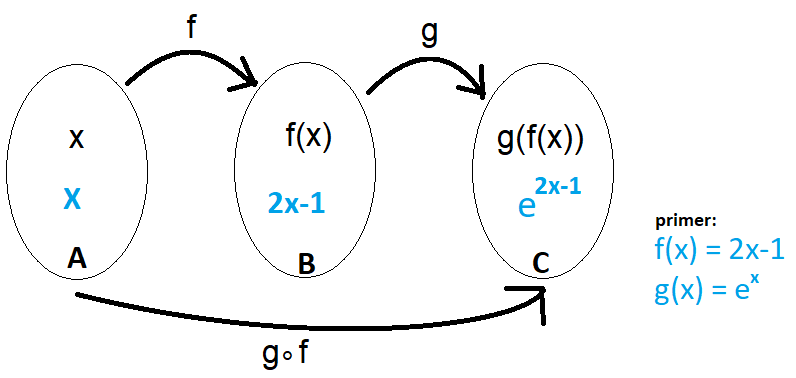
\includegraphics[width=0.7\textwidth]{slike/kompozitum.png}
\end{figure*}

\vaje{
Vaje:
\begin{itemize}
    \item Preproste vaje, kjer iz sestavljene funkcije ugotavljajo, katera je zunanja ($ g $) in katera notranja ($ f $)
    \item kompozitum $ f $ in njenega inverza je $ x \mapsto x $
    \item iz danih $ f $ in $ g $ računajo $ f \circ g $ in $ g \circ f $ ipd.
\end{itemize}
}

    
\end{priprava}